

\documentclass{beamer}
\beamertemplatenavigationsymbolsempty
\usecolortheme{beaver}
\setbeamertemplate{blocks}[rounded=true, shadow=true]
\setbeamertemplate{footline}[page number]
%
\usepackage[utf8]{inputenc}
\usepackage[english,russian]{babel}
\usepackage{amssymb,amsfonts,amsmath,mathtext}
\usepackage{subfig}
\usepackage[all]{xy} % xy package for diagrams
\usepackage{array}

\usepackage[sorting=none]{biblatex} %Imports biblatex package
\addbibresource{biblio.bib}

\usepackage{multicol}% many columns in slide
\usepackage{hyperref}% urls
\usepackage{hhline}%tables
% Your figures are here:
\graphicspath{ {figures/} {../figures/} }

%----------------------------------------------------------------------------------------------------------

\newtheorem{mytheorem}{\color{black} \textbf{Теорема}}
\newtheorem{mydefinition}{Определение}
\newtheorem{myexample}{\color{orange}Пример}
% \newcommand{\mbR}{\mathbb{R}}
% \newcommand\marker[2]{{\fboxsep=0pt\colorbox{#1}{\strut #2}}}
\newcommand{\marker}[2]{\textcolor{#1}{#2}}
% \newcommand{\clip}{\texttt{clip}}
% \newcommand{\tvi}{f_i(x_i)}
\usepackage{tikz}

\newcommand{\titleName}{Stein variatonal GD \\ vs \\ black-box variational inference}
%----------------------------------------------------------------------------------------------------------
\title[\hbox to 56mm{\titleName}]{\titleName}
\institute{Кафедра Интеллектуальных систем МФТИ}
\author[И.\,М.~Латыпов]{И.\,М.~Латыпов}
\date{2024}

%----------------------------------------------------------------------------------------------------------
\begin{document}
\begin{frame}
\thispagestyle{empty}
\maketitle
\end{frame}


\begin{frame}{About paper}
    Motivation:  There are two popular methods for Bayesian inference: Stein variational gradient descent (SVGD)\cite{liu2016stein} and black-box variational inference (BBVI). Are they equivalent on some meanings?

    \par
    PLAN:
    \begin{enumerate}
        \item  Stein variational gradient descent (SVGD).
        \item  Black-box variational inference (BBVI).
        \item  Equivalence demonstration.
    \end{enumerate}
    
    \noindent\makebox[\linewidth]{\rule{\paperwidth}{0.4pt}}
    Results: BBVI corresponds precisely to SVGD when the kernel is the neural tangent kernel. \\
    \textcolor{red}{Interpretation of SVGD and BBVI as kernel gradient flows and their connectivity with GANs}.
    
\end{frame}

\begin{frame}{SVGD}
Notations:
\begin{enumerate}
    \item  Let $p(x), q(x)$ be a continuously differentiable  density, supported on $\mathcal{X} \subseteq \mathbb{R}^d$.
    \item $\phi(x): \mathbb{R}^d \rightarrow \mathbb{R}^d$ -- smooth vector function.    
\end{enumerate}
Then \textbf{Stein`s Identity} is satisfied:

\begin{align}
&\mathbb{E}_{x\sim p} \mathcal{A}_p(x) = 0, \\
&\mathcal{A}_p(x) = \phi(x)\nabla_x \log p(x)^T + \nabla_x \phi(x).
\end{align}

HINT: take the derivative of the mathematical expectation.

Define \textbf{Stein discrepancy}:
\begin{equation}
\mathbb{S}(q, p) = \max_{f\in \mathcal{F}}\left\{ \left[\mathbb{E}_{x\sim \color{red} q} \text{trace}(\mathcal{A}_{ \color{blue} p}\phi(x))\right]^2 \right\}
\end{equation}

\end{frame}

\begin{frame}{SVGD}
    Kernelized Stein discrepancy on reproducing kernel Hilbert space $\mathcal{H}^d$ by Liu et al. \cite{liu2016kernelized}:
    \begin{equation}
\mathbb{S}(q, p) = \max_{f\in \mathcal{H}^d}\left\{ \left[\mathbb{E}_{x\sim \color{red} q} \text{trace}(\mathcal{A}_{ \color{blue} p}\phi(x))\right]^2 ~~ s.t. \|\phi\|_{\mathcal{H}^d} \leq 1 \right\}.
\end{equation}

 \textbf{The point:} there is \textit{kernel} $k(x, x`)$ in $\mathcal{H}^d$, and we can find optimal solution.
\begin{align}
    &\phi(x) = \phi^*_{q,p}(x)/ \|\phi^*_{q,p}(x)\|_{\mathcal{H}^d}, \\
    &\phi^*_{q,p}(\cdot) = \mathbb{E}_{x\sim q} [\mathcal{A}_p k(x, \cdot )]\\
    \mathbb{S}(q, p)&= \|\phi^*_{q,p}(x)\|_{\mathcal{H}^d}.
\end{align}
\end{frame}

\begin{frame}{Var inference with Smooth Transforms}
\begin{equation}
    q^* = \text{arg} \min_{q \in \mathcal{Q}} \left\{ \text{KL}(q || p) \equiv \mathbb{E}_q[\log q(x) - p(x)p(D|x)] + C )\right\}
\end{equation}

Consider $\mathcal{Q}$ as a small evolutions:

\begin{align}
    &x \sim q(x) \\
    &z = T(x) = x + \epsilon \phi(x)
\end{align}
\begin{figure}
    \centering
    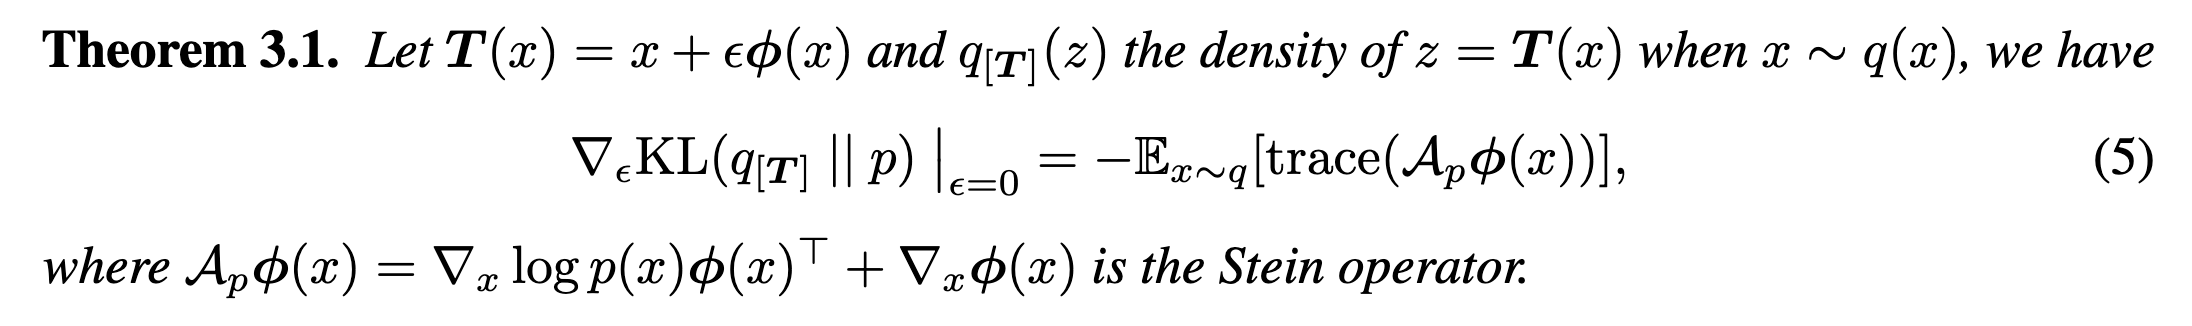
\includegraphics[width=1\linewidth]{figures/theorem.png}
\end{figure}
\end{frame}

\begin{frame}{SVGD}
\begin{figure}
    \centering
    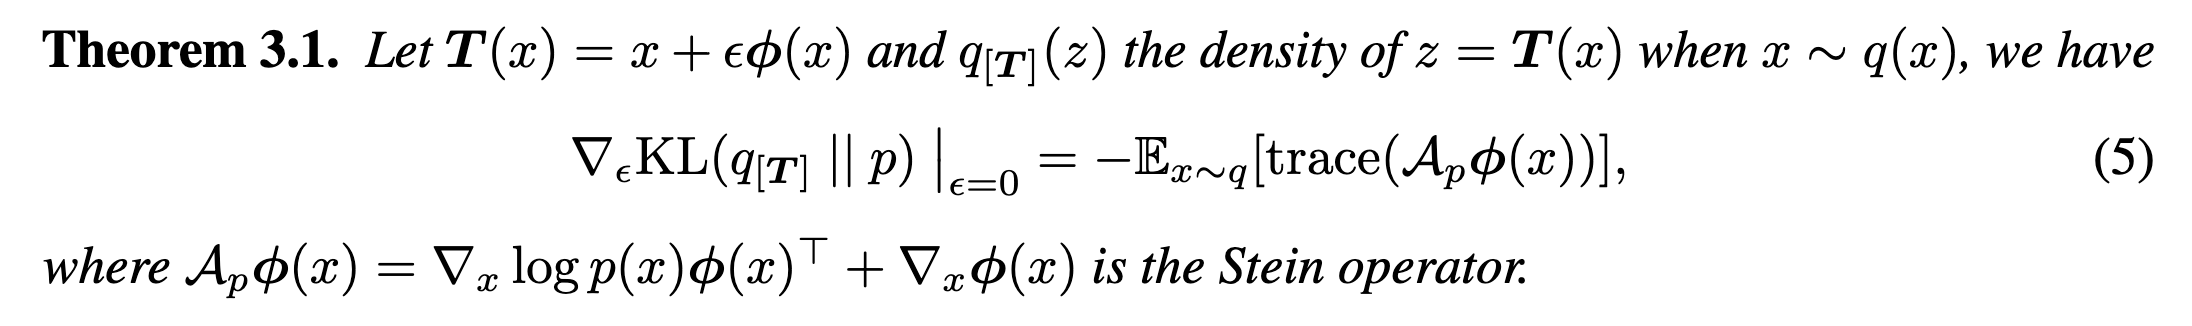
\includegraphics[width=1\linewidth]{figures/theorem.png}
\end{figure}
    \begin{figure}
    \centering
    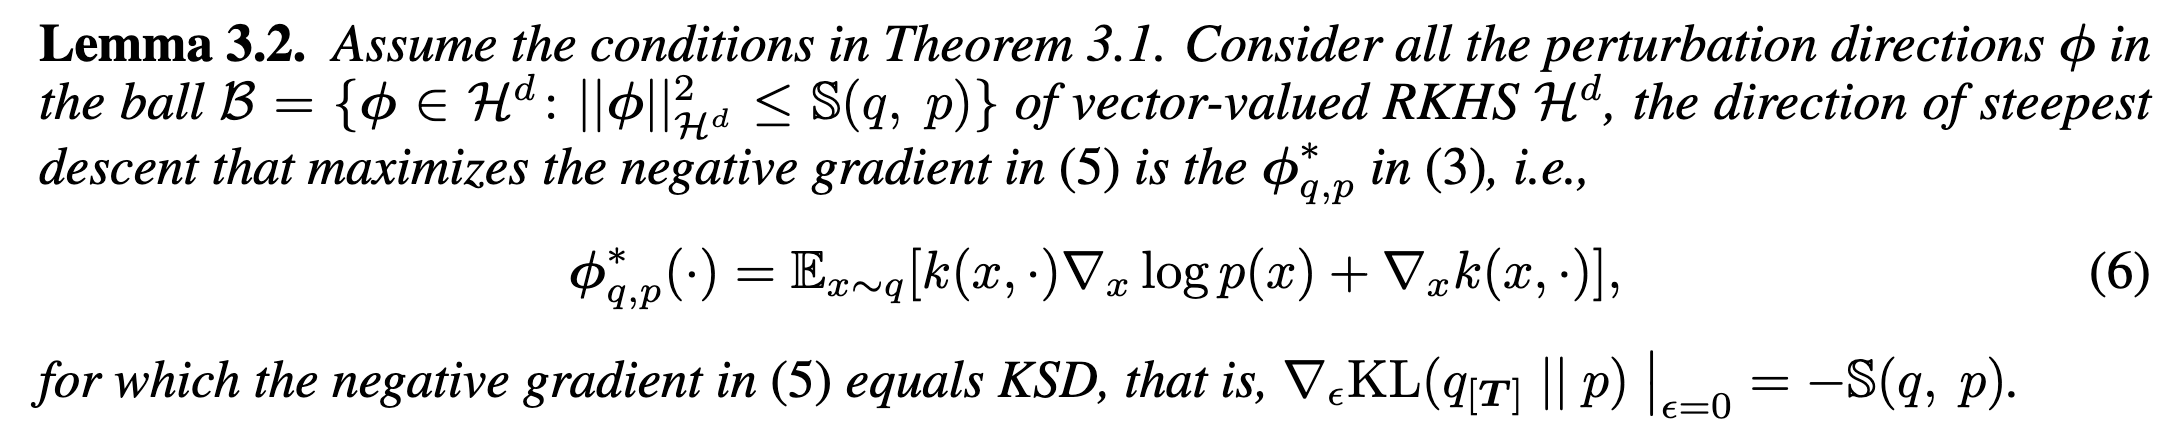
\includegraphics[width=1\linewidth]{figures/lemma.png}
\end{figure}

\begin{align}
    &T^*(x)_l = x + \epsilon_l \cdot \phi^*_{q_l, p}(x)\\
    &q_{l+1} = T^*_l(q_l)
\end{align}

\end{frame}

\begin{frame}{SVGD algorithm}
    \begin{figure}
        \centering
        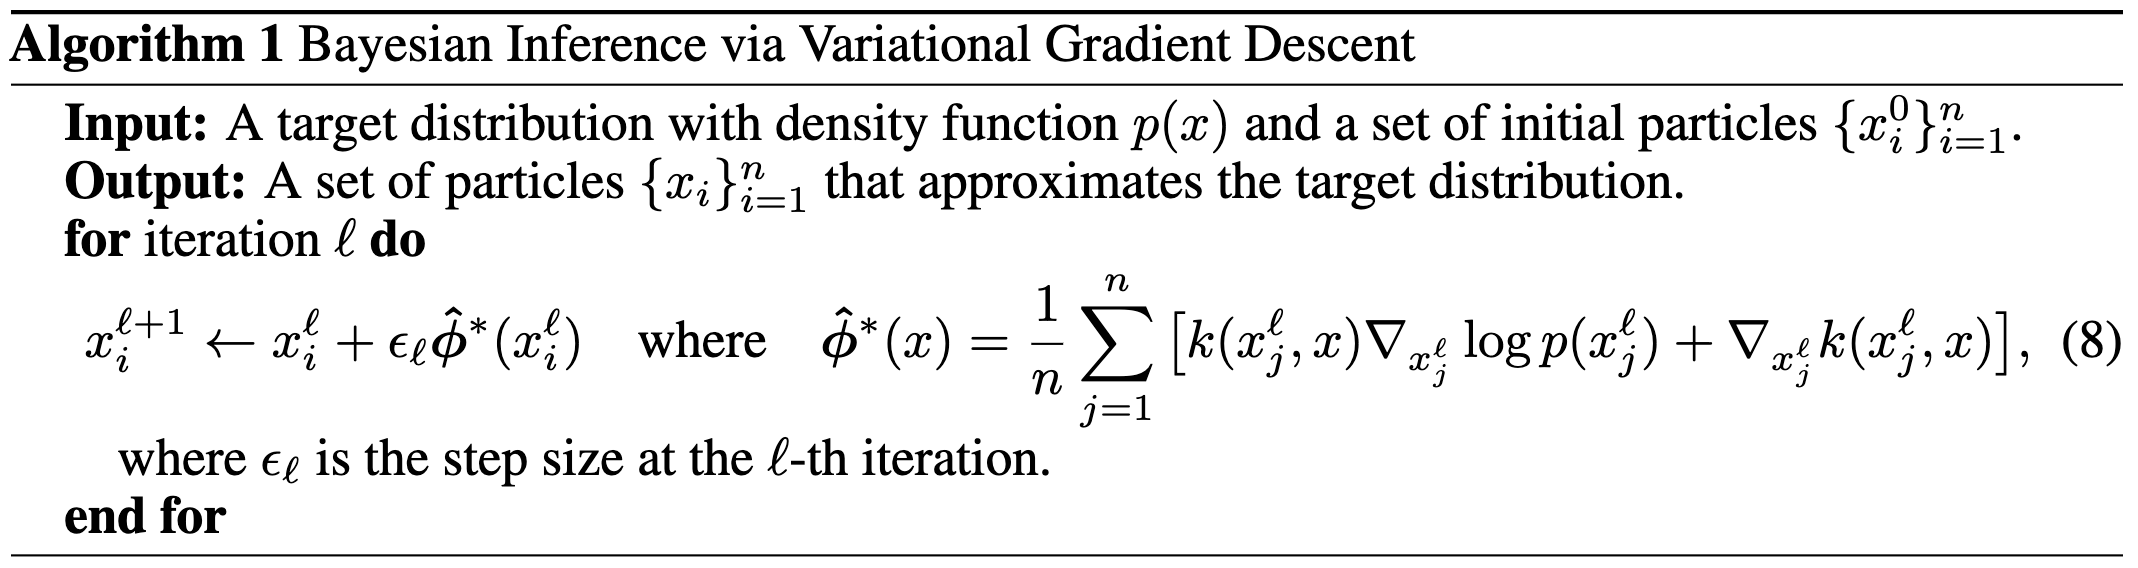
\includegraphics[width=\linewidth]{figures/algorithm.png}
    \end{figure}
    \begin{figure}
        \centering
        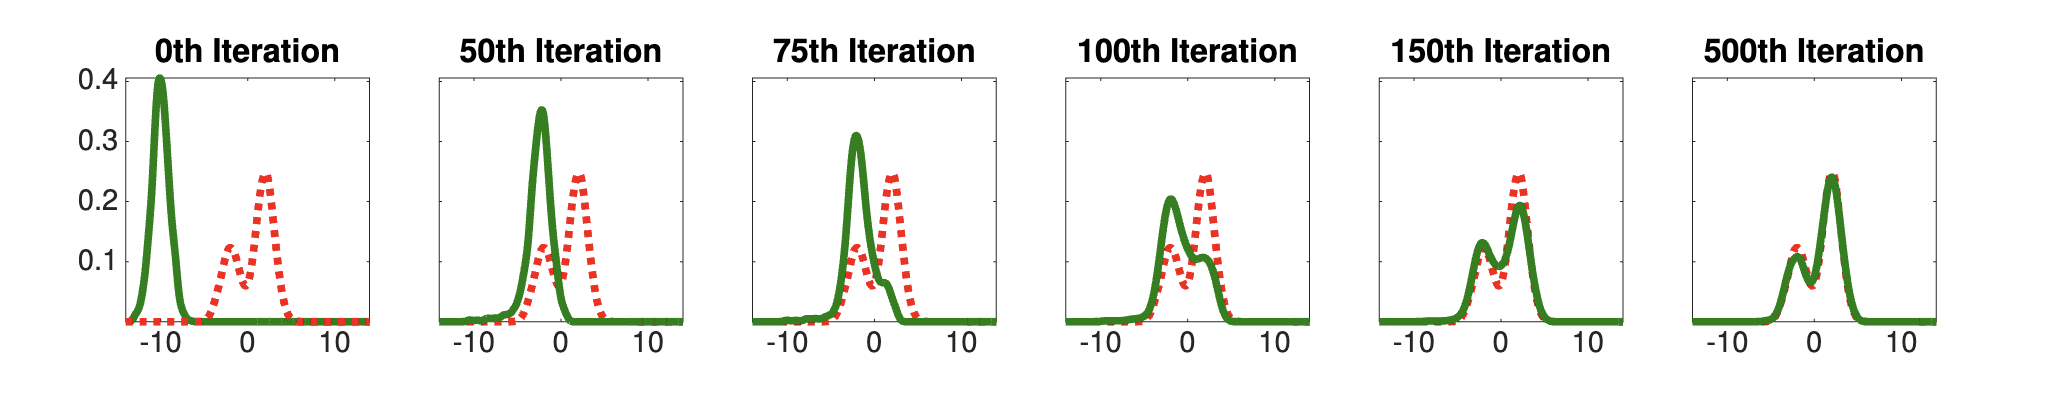
\includegraphics[width=0.9\linewidth]{figures/experiment.png}
        \caption{The red dashed lines are the target density function
and the solid green lines are the densities of the particles at different iterations of algorithm.}
        \label{fig:enter-label}
    \end{figure}
    
\end{frame}

\begin{frame}{SVGD integral form}
    \begin{align}
        \frac{dx_i}{dt} = &\mathbb{E}_{y \sim q_t} [k(x_i, y) \nabla_y\log p(y) + \nabla_y k(x_i, y)] \\
        &q_t = \frac{1}{n}\sum^n_{i=1} \delta_{x_i(t)}
    \end{align}

In limit it is equivalent to \cite{lu2019scaling}:
    \begin{align}
        \frac{dx}{dt} = &\mathbb{E}_{y \sim q_t} [{\color{blue} k(x, y)} \nabla_y {\color{red}(} \log p(y) - \log q_t(y) {\color{red})}] \\
    \end{align}

\end{frame}

\begin{frame}{BBox variational inference}
 ELBO maximization:
 \begin{align}
     L(\phi) :=\mathbb{E}_{x \sim q_\phi} \left[ \log\frac{P(D|x)P(x)}{q_\phi(x)}\right], \\
     \text{KL}(q_{\phi}(x)|| p(x)) = P(z) - L(\phi) \rightarrow \min.
 \end{align}
$\phi$ dynamics:
\begin{equation}
    \frac{d\phi}{dt} = \nabla_{\phi}L(\phi).
\end{equation}

 To get derivative we use reparametrization trick by Kingma:
\begin{equation}
    x \sim q_{\phi} \Longleftrightarrow \varepsilon \sim \omega ~\text{and}~ x = f_{\phi}(\varepsilon).
\end{equation}

According to \cite{liu2016kernelized}:
\begin{equation}
    \nabla_{\phi}L(\phi) = \mathbb{E}_{w \sim \omega} \nabla_\phi f_\phi(w)\cdot \nabla_y
    (\log(p(y) - \log(q_\phi(y))|_{y = f_\phi(w)}
\end{equation}
\end{frame}

\begin{frame}{BBox variational inference}
    We can get derivative $dx/dt$:
    \begin{align}
        \frac{dx}{dt}& =(\nabla_\phi f_\phi(\varepsilon))^T \frac{d\phi}{dt}=\\
        &\mathbb{E}_{w \sim \omega} {\color{blue} \nabla_\phi f_\phi(\varepsilon)^T \nabla_\phi f_\phi(w)}\cdot \nabla_y (\log(p(y) - \log(q_\phi(y))|_{y = f_\phi(w)} 
    \end{align}
    Let's introduce \textit{neural tangent kernel} \cite{jacot2018neural}:
    \begin{align}
        \Theta_\phi(\varepsilon, w) := {\color{blue} \nabla_\phi f_\phi(\varepsilon)^T \nabla_\phi f_\phi(w)} \\
        k_\phi(x, y) := \Theta_\phi(f_\phi^{-1}(\varepsilon), f_\phi^{-1}(w))
    \end{align}

Finalle::
    $$
        \frac{dx}{dt} = \mathbb{E}_{y \sim q_t} [{\color{blue} k(x, y)} \nabla_y {\color{red}(} \log p(y) - \log q_t(y) {\color{red})}]
    $$
    
\end{frame}

\begin{frame}{Summary}
\begin{enumerate}
    \item Reviewed SVGD method.
    \item Repeated what BBVI does and found its derivatives.
    \item Show, that SVGD distribution evolution with \textit{neural tangent kenel} is equivalent to BBVI.
\end{enumerate}    
\end{frame}
\begin{frame}{finalle}
    % \bibliography{biblio}
    \printbibliography
\end{frame}
\end{document} 